%%%%%%%%%%%%%%%%%%%%%%%%%%%%%%%%%%%%%%%%
%%%%%%% created by Attila Karsai %%%%%%%
%%%%%%%                          %%%%%%%
%%%%%%% by default, the template %%%%%%%
%%%%%%%    only compiles using   %%%%%%%
%%%%%%%   lualatex. if you dont  %%%%%%%
%%%%%%% have lualatex installed, %%%%%%%
%%%%%%% just uncomment the lines %%%%%%%
%%%%%%%%%%%%%%%%%%%%%%%%%%%%%%%%%%%%%%%%
%%%% if you have problems/questions %%%%
% contact me: karsai@math.tu-berlin.de %
%%%%%%%%%%%%%%%%%%%%%%%%%%%%%%%%%%%%%%%%

%  changelog:
%  - 2024-jan-26
%     - removed external commands file
%     - changed folder structure
%     - added commands to fix spacing issues with monospaced fonts
%     - added section command in beamertheme_FGMSO.sty
%     - improved documentation a bit
% - 2023-jan-21
%     - first release

%%%%%%%%%%%%%%%%%%%%%%%%%%%%%%%%%%%%%%%%

\documentclass[aspectratio=169,mathserif,noamsthm,13pt]{beamer}

\usepackage[english]{babel}
\usepackage{csquotes}

%%%%%%%%%%%%%%%%%%%%%%%%%%%%%%%%%%%%%%%%
%%%%%% for LuaLaTeX and JuliaMono %%%%%%
%%%%%%%%%%%%%%%%%%%%%%%%%%%%%%%%%%%%%%%%

%\usepackage{fontspec}
%    \defaultfontfeatures{Scale=0.9}
    %\setmonofont{JuliaMono}
    %\setmonofont{Menlo}

%%%%%%%%%%%%%%%%%%%%%%%%%%%%%%%%%%%%%%%%
%%%%%% for pdfLaTeX and BeraMono %%%%%%%
%%%%%%%%%%%%%%%%%%%%%%%%%%%%%%%%%%%%%%%%
\usepackage[utf8]{inputenc}
\usepackage[T1]{fontenc}
\usepackage{yfonts}
\usepackage[scaled]{beramono}
\usepackage[sfdefault]{inter}


%%%%%%%%%%%%%%%%%%%%%%%%%%%%%%%%%%%%%%%%
%%%%% to fix spacing of mono fonts %%%%%
%%%%%%%%%%%%%%%%%%%%%%%%%%%%%%%%%%%%%%%%
\usepackage{everysel}
    \EverySelectfont{%
    \fontdimen2\font=0.4em% interword space
    \fontdimen3\font=0.2em% interword stretch
    \fontdimen4\font=0.1em% interword shrink
    \fontdimen7\font=0.1em% extra space
    \hyphenchar\font=`\-% to allow hyphenation
}
\usepackage{microtype}


\usepackage{pgfplots}
\usepackage{tikz}
\pgfplotsset{compat=newest}
    \usetikzlibrary{plotmarks}
    \usetikzlibrary{calc}
    \usetikzlibrary{positioning}
    \usetikzlibrary{arrows.meta}
    \usetikzlibrary{matrix}
    \usepgfplotslibrary{patchplots}
    \usetikzlibrary{shapes.geometric, arrows}
    
    \tikzstyle{startstop} = [rectangle, rounded corners, 
    minimum width=3cm, 
    minimum height=1cm,
    text centered, 
    draw=black, 
    fill=alertcolor]
    
    \tikzstyle{code} = [rectangle, 
    minimum width=3cm, 
    minimum height=1cm, 
    text centered, 
    draw=black, 
    ]
    
    \tikzstyle{decision} = [diamond, 
    minimum width=3cm, 
    minimum height=1cm, 
    text centered, 
    draw=black, 
    fill=green!30]
    \tikzstyle{arrow} = [thick,->,>=stealth]
\usepackage[framemethod=TikZ]{mdframed}
\usepackage{xstring}
\usepackage{etoolbox}
\usepackage{ifthen}
\usepackage[shortlabels]{enumitem}

\usepackage{amsmath}
\usepackage{amssymb}
\usepackage{amsthm}
% \usepackage{thmtools}

% \usepackage{pdfpages}
\usepackage{xspace}
\usepackage{graphicx}
    \graphicspath{.}

\usepackage[labelsep=period]{caption}
    \captionsetup[figure]{font=small,width=.9\linewidth,belowskip=-7pt}

\usepackage[style=ieee]{biblatex}
\usepackage{bibentry}
\addbibresource{Bibliography.bib}

% For \Verb
\usepackage{fancyvrb}
% For pseudocode
\usepackage[noend]{algorithm2e}






%%%%%%%%%%%%%%%%%%%%%%%%%%%%%%%%%%%%%%%%
%%%%%%%%%%%%%%%% colors %%%%%%%%%%%%%%%%
%%%%%%%%%%%%%%%%%%%%%%%%%%%%%%%%%%%%%%%%
%%% the alertcolor is the main color %%%
%%%%%% of the entire presentation %%%%%%
%%%%%%%%%%%%%%%%%%%%%%%%%%%%%%%%%%%%%%%%
%\definecolor{alertcolor}{RGB}{55, 107, 140}  % blue, default
\definecolor{alertcolor}{cmyk}{0.85,0.21,0,0} % Aalto blue
\definecolor{lesscolor}{RGB}{43,58,68} % Original structure

% \definecolor{alertcolor}{RGB}{186, 137, 0} % orange
% \definecolor{alertcolor}{RGB}{108, 0, 140} % purple
% \definecolor{alertcolor}{RGB}{15, 135, 0}  % green
% \definecolor{alertcolor}{RGB}{197, 14, 31} % TUB red
%\definecolor{examplecolor}{RGB}{15, 102, 0}
\definecolor{examplecolor}{cmyk}{0, 59, 80, 0} % Aalto Orange
\setbeamercolor{alerted text}{fg=alertcolor}
\setbeamercolor{block title alerted}{bg=alertcolor}


%%%%%%%%%%%%%%%%%%%%%%%%%%%%%%%%%%%%%%%
%%%%%%%%%%%%% custom boxes %%%%%%%%%%%%
%%%%%%%%%%%%%%%%%%%%%%%%%%%%%%%%%%%%%%%
% no thmtools

% decide if plain theorems should be numbered (theorems, lemmas, ...)
\newcommand{\plainnumbered}{0} % 1 - numbered, 0 - unnumbered
\newcounter{plain}
\setcounter{plain}{1}

% decide if vari thms should be numbered (examples ...)
\newcommand{\varinumbered}{0} % 1 - numbered, 0 - unnumbered
\newcounter{vari}
\setcounter{vari}{1}

% this command defines a command to define theorems, lemmas, etc.
% \makeatletter
\newcommand{\defineplaintheorem}[3][alertcolor]{
    \newenvironment{#2}[1][\@nil]
        {%
        \def\tmp{##1}%
        \ifthenelse{\equal{##1}{\@nil}}
            {\ifnum\plainnumbered=0 % and no numbering is wished for
                            \def\frmtitle{\color{#1}\bfseries #3.}
                        \else % if numbering is wished
                            \def\frmtitle{\color{#1}\bfseries #3
                            \arabic{plain}\stepcounter{plain}.}
                        \fi}
            {\ifnum\plainnumbered=0 % and no numbering is wished for
                            \def\frmtitle{\color{#1}\bfseries #3 \mdseries[##1]\bfseries.}
                        \else % if numbering is wished
                            \def\frmtitle{\color{#1}\bfseries #3 \arabic{plain}\stepcounter{plain} \mdseries[##1]\bfseries.}
                        \fi}
        \color{black} % dirty fix!
        \normalsize % dirty fix!
        \begin{mdframed}[
            roundcorner=2pt,
            backgroundcolor=white!90!#1,
            linecolor=#1,
            linewidth=.7pt, 
            % linewidth=0pt, 
            frametitle={\frmtitle},
            frametitlebelowskip=2pt,
            innertopmargin=2pt,
            % frametitlerule=true,
            % frametitlebackgroundcolor=#1!25!white,
            ]
        % \tolerance 2000%
        % \emergencystretch 3em%
        % \hfuzz .5\p@
        % \vfuzz\hfuzz
        }
        {
        \end{mdframed}
        }
}


\newcommand{\definevaritheorem}[3][examplecolor]{
    \newenvironment{#2}[1][\@nil]
        {
        \def\tmp{##1}%
        \ifx\tmp\@nnil % if no name of the theorem is given
            \ifnum\varinumbered=0 % and no numbering is wished for
                \def\frmtitle{\color{#1}\bfseries #3.}
            \else % if numbering is wished
                \def\frmtitle{\color{#1}\bfseries #3
                \arabic{vari}\stepcounter{vari}.}
            \fi
        \else % if theorem name is given
            \ifnum\varinumbered=0 % and no numbering is wished for
                \def\frmtitle{\color{#1}\bfseries #3 \mdseries[##1]\bfseries.}
            \else % if numbering is wished
                \def\frmtitle{\color{#1}\bfseries #3 \arabic{vari}\stepcounter{vari} \mdseries[##1]\bfseries.}
            \fi
        \fi
        \begin{mdframed}[
            roundcorner=2pt,
            backgroundcolor=white!90!#1,
            % linecolor=green,
            linewidth=0pt,
            frametitle={\frmtitle},
            frametitlebelowskip=2pt,
            innertopmargin=2pt,
            % frametitlerule=true,
            % frametitlebackgroundcolor=alertcolor!10!white,
            ]
        % \tolerance 2000%
        % \emergencystretch 3em%
        % \hfuzz .5\p@
        % \vfuzz\hfuzz
        }
        {
        \end{mdframed}
        }
}
% \makeatother






%--------- for thmtools --------
% \def \leftrightmargin {20}
%
% \makeatletter
% % a robust wrapper of \qedsymbol
% \protected\edef\xqedsymbol{\unexpanded\expandafter{\qedsymbol}}
% \makeatother
%
%
%
% % only used for remark
% \declaretheoremstyle[
% spaceabove=0pt, spacebelow=0pt,
% headfont=\normalfont\bfseries,
% notefont=\mdseries, notebraces={(}{)},
% bodyfont=\small\normalfont,
% postheadspace=1em,
% mdframed={innertopmargin=0pt,
%           innerbottommargin=0pt,
%           innerleftmargin=\leftrightmargin pt,
%           innerrightmargin=\leftrightmargin pt,
%           hidealllines=true,
%           }
% ]{standardrem}
%
% % only used for example
% \declaretheoremstyle[
% spaceabove=0pt, spacebelow=0pt,
% headfont=\normalfont\bfseries,
% notefont=\mdseries, notebraces={(}{)},
% bodyfont=\small\normalfont,
% postheadspace=1em,
% mdframed={innertopmargin=0pt,
%           innerbottommargin=0pt,
%           innerleftmargin=\leftrightmargin pt,
%           innerrightmargin=\leftrightmargin pt,
%           hidealllines=true,
%           }
% ]{standardex}
%
% % this is used for theorems, lemmas, corollarys
% \declaretheoremstyle[
% spaceabove=3pt, spacebelow=0pt,
% headfont=\color{alertcolor}\bfseries,
% notefont=\color{alertcolor}\mdseries, notebraces={[}{]},
% bodyfont=\normalfont,
% postheadspace=\newline,
% mdframed={
%             backgroundcolor=alertcolor!10!white,
%             linewidth=0pt,
%             roundcorner=3pt,
%           }
% ]{standarddef}
%
% % only used for proof
% \declaretheoremstyle[
% spaceabove=0pt, spacebelow=0pt,
% headfont=\normalfont\itshape,
% bodyfont=\normalfont,
% postheadspace=1em,
% qed=$\blacksquare$,
% mdframed={innertopmargin=0pt,
%           innerbottommargin=0pt,
%           innerleftmargin=\leftrightmargin pt,
%           innerrightmargin=\leftrightmargin pt,
%           skipabove=-10pt,
%           hidealllines=true,
%           }
% ]{standardproof}
%
% \declaretheorem[
% style=standarddef,
% refname={Theorem,Theorems},
% Refname={Theorem,Theorems}]{theorem}
%
% \declaretheorem[
% style=standarddef,
% sibling=theorem,
% refname={Lemma,Lemmas},
% Refname={Lemma,Lemmas}]{lemma}
%
% \declaretheorem[
% style=standarddef,
% sibling=theorem,
% refname={Corollary,Corollarys},
% Refname={Corollary,Corollarys}]{corollary}
%
% \declaretheorem[
% style=standarddef,
% sibling=theorem,
% refname={Definition,Definitions},
% Refname={Definition,Definitions}]{definition}
%
% \declaretheorem[
% style=standardrem,
% sibling=theorem,
% refname={Remark,Remarks},
% Refname={Remark,Remarks}]{remark}
%
% \declaretheorem[
% style=standardex,
% sibling=theorem,
% refname={Example,Examples},
% Refname={Example,Examples}]{example}
    % better not change this...


% here, the theorem and lemmas are defined.
% the syntax is
%   \defineplaintheorem[background color]{environment name}{title shown in bold}
%
\defineplaintheorem{theorem}{Theorem}
\defineplaintheorem{lemma}{Lemma}
\defineplaintheorem{proposition}{Proposition}
\defineplaintheorem{corollary}{Corollary}
\defineplaintheorem{definition}{Definition}
\defineplaintheorem[examplecolor]{example}{Example}
\defineplaintheorem[examplecolor]{assumption}{Assumption}

% there is also a second environment defined, which allows
% to, e.g., number examples differently. the syntax is the same.
%   an example is:
%
% \definevaritheorem{example}{Example}



%%%%%%%%%%%%%%%%%%%%%%%%%%%%%%%%%%%%%%%
%%%%%%%%%%% custom commands %%%%%%%%%%%
%%%%%%%%%%%%%%%%%%%%%%%%%%%%%%%%%%%%%%%
\newcommand{\RR}{\mathbb{R}}
\newcommand{\CC}{\mathbb{C}}
\newcommand{\norm}[1]{\Vert #1 \Vert}
\newcommand{\sca}[1]{\langle #1 \rangle}
\newcommand{\scal}[2]{\langle #1, #2 \rangle}
% \newcommand{\wip}{\color{black!30!red}}
\newcommand{\inv}{^{-1}}
\newcommand{\tp}{^{\mathsf{T}}}
\newcommand{\herm}{^{\mathsf{H}}}
\newcommand*\dif{\mathop{}\!\mathrm{d}}

% \newcommand{\dt}{\,\mathrm{d}t}
\newcommand{\missing}{\wip missing. \color{black}}
\renewcommand{\vec}[1]{\begin{bmatrix} #1 \end{bmatrix}}
\newcommand{\fApp}{\boldsymbol{\mathfrak{f}}}

\def\divdif{{\vrule\mkern-8mu \Delta}}

%%%%%%%%%%%%%%%%%%%%%%%%%%%%%%%%%%%%%%%%
%%%%%%%%%%%%% nice := sign %%%%%%%%%%%%%
%%%%%%%%%%%%%%%%%%%%%%%%%%%%%%%%%%%%%%%%
\mathchardef\ordinarycolon\mathcode`\:
\mathcode`\:=\string"8000
\begingroup \catcode`\:=\active
  \gdef:{\mathrel{\mathop\ordinarycolon}}
\endgroup


%%%%%%%%%%%%%%%%%%%%%%%%%%%%%%%%%%%%%%%%
%%%%%%%%%% nice mathcal font %%%%%%%%%%%
%%%%%%%%%%%%%%%%%%%%%%%%%%%%%%%%%%%%%%%%
\DeclareMathAlphabet{\altmathcal}{OMS}{cmsy}{m}{n}
\renewcommand{\mathcal}{\altmathcal}


%%%%%%%%%%%%%%%%%%%%%%%%%%%%%%%%%%%%%%%%
%%%%%%%%% custom cite command %%%%%%%%%%
%%%%%%%%%%%%%%%%%%%%%%%%%%%%%%%%%%%%%%%%
\newcommand{\mycitestyle}{\color{alertcolor}}
\newcommand{\mycitestyletiny}{\color{lesscolor}\tiny}
\makeatletter
\def\blfootnote{\xdef\@thefnmark{}\@footnotetext}
\makeatother
\let\oldcite\cite
\newcommand{\fakeAuthoYearCite}[1]{\citeauthor{#1} (\citeyear{#1}). \citetitle{#1}.}
\newcommand{\footnoteCiteStyle}[1]{{\color{alertcolor}\oldcite{#1}} \fakeAuthoYearCite{#1}}
\renewcommand{\cite}[1]{{\mycitestyle\oldcite{#1}}\blfootnote{\mycitestyletiny\footnoteCiteStyle{#1}}}

\newcommand{\dcite}[2]{{\oldcite{#1, #2}}
%\blfootnote{\mycitestyletiny {\color{alertcolor}\oldcite{#1}} \fakeAuthoYearCite{#1}}
%\blfootnote{\mycitestyletiny {\color{alertcolor}\oldcite{#2}} \fakeAuthoYearCite{#2}}
}

% \newcommand{\dcite}[2]{{\mycitestyle\oldcite{#1,#2}}\blfootnote{\mycitestyletiny\oldcite{#1}~\bibentry{#1}}\blfootnote{\mycitestyletiny\oldcite{#2}~\bibentry{#2}}}

% \newcommand{\blfootcite}[1]{\blfootnote{\mycitestyletiny\oldcite{#1}~\bibentry{#1}}}

% \newcommand{\ifootcite}[1]{\mycitestyle\color{white}\oldcite{#1}\blfootnote{\mycitestyletiny\color{white}\oldcite{#1}~\bibentry{#1}}}

% \newcommand{\framecite}[2]{\SUBTRACT{#2}{1}{\citevisible}\only<#2->{\cite{#1}}\only<-\citevisible>{\ifootcite{#1}}}


%%%%%%%%%%%%%%%%%%%%%%%%%%%%%%%%%%%%%%%%
%%%%%%%%%%%% tikz functions %%%%%%%%%%%%
%%%%%%%%%%%%%%%%%%%%%%%%%%%%%%%%%%%%%%%%
\makeatletter
\newcommand{\gettikzxy}[3]{%
  \tikz@scan@one@point\pgfutil@firstofone#1\relax
  \edef#2{\the\pgf@x}%
  \edef#3{\the\pgf@y}%
}
\makeatother


%%%%%%%%%%%%%%%%%%%%%%%%%%%%%%%%%%%%%%%%
%%%%%%%%%% underfull box fix %%%%%%%%%%%
%%%%%%%%%%%%%%%%%%%%%%%%%%%%%%%%%%%%%%%%
\emergencystretch=3em
\hbadness=99999  % or any number >=10000


%%%%%%%%%%%%%%%%%%%%%%%%%%%%%%%%%%%%%%%%
%%%%%%%%%%% vspace shortcuts %%%%%%%%%%%
%%%%%%%%%%%  -come in handy- %%%%%%%%%%%
%%%%%%%%%%%%%%%%%%%%%%%%%%%%%%%%%%%%%%%%
\newcommand{\vs}{\vspace{0.5cm}}
\newcommand{\vsm}{\vspace{-0.3cm}}


%%%%%%%%%%%%%%%%%%%%%%%%%%%%%%%%%%%%%%%%
%%%%%%%%%%%% itemize symbol %%%%%%%%%%%%
%%%%%%%%%%%%%%%%%%%%%%%%%%%%%%%%%%%%%%%%
\newcommand{\isym}{\tiny\raisebox{1.5pt}{$\blacksquare$}}
% \newcommand{\isym}{-} % a more traditional item style
\setlist[itemize]{label=\isym}


%%%%%%%%%%%%%%%%%%%%%%%%%%%%%%%%%%%%%%%%
%%%%%%% your image files go here %%%%%%%
%%%%%%%%%%%%%%%%%%%%%%%%%%%%%%%%%%%%%%%%
%\newcommand{\institutegraphic}{resources/tub-logo.jpg}
\newcommand{\institutegraphic}{} % no institute graphic

% \newcommand{\projectgraphic}{resources/trr-logo.png} % trr logo
%\newcommand{\projectgraphic}{resources/daedalus-logo.png} % daedalus logo
\newcommand{\projectgraphic}{} % no project graphic

%\newcommand{\fundinggraphic}{resources/wide_blue_title.png}
\newcommand{\fundinggraphic}{} % no funding graphic


%%%%%%%%%%%%%%%%%%%%%%%%%%%%%%%%%%%%%%%%
%%%%%%%%%%%% image heights %%%%%%%%%%%%%
%%%%%%%%%%%%%%%%%%%%%%%%%%%%%%%%%%%%%%%%
\newcommand{\instituteheight}{.3\textheight}
\newcommand{\projectheight}{.18\textheight}
\newcommand{\fundingheight}{\textheight}


%%%%%%%%%%%%%%%%%%%%%%%%%%%%%%%%%%%%%%%%
%%%% tell latex to use beamertheme %%%%%
%%%%%%%%%%%%%%%%%%%%%%%%%%%%%%%%%%%%%%%%
\usetheme{FGMSO}


%%%%%%%%%%%%%%%%%%%%%%%%%%%%%%%%%%%%%%%%
%%%%%% typewriter font as default %%%%%%
%%%%%%%%%%%%%%%%%%%%%%%%%%%%%%%%%%%%%%%%
%\renewcommand{\familydefault}{\ttdefault}


%%%%%%%%%%%%%%%%%%%%%%%%%%%%%%%%%%%%%%%%
%%%%%%%%%%%% talk metadata %%%%%%%%%%%%%
%%%%%%%%%%%%%%%%%%%%%%%%%%%%%%%%%%%%%%%%

\title[Large Scale Data Engineering Seminar]{\LARGE Optimizing Code Generation for Matrix Multiplication}
\subtitle{DAPHNE}
\author[H. Willems]{Henri Willems
\\ \normalfont %\ttfamily
henri.willems@campus.tu-berlin.de
}
\institute[TU Berlin]{WS 23/24, TU Berlin}
\date{March 04, 2024}











%%%%%%%%%%%%%%%%%%%%%%%%%%%%%%%%%%%%%%%%
%%%%%%%%%% action starts here %%%%%%%%%%
%%%%%%%%%%%%%%%%%%%%%%%%%%%%%%%%%%%%%%%%

\begin{document}




\begin{frame}[noframenumbering,plain]
    \maketitle
    
\end{frame}


\begin{frame}{Matrix Multiplication Implementation}
    Matrix Multiplication is Level 3 Basic Linear Algebra Subprogram \cite{dongarra_blas} operation\vs

    Hardware specific hand optimization, e.g. Intel oneMKL BLAS \cite{intelrAccelerateFastMath}\vs
    
    Daphne uses BLIS \cite{BLIS1} a ``portable software framework for instantiating high-performance BLAS-like dense linear algebra libraries''\vs

    \pause
    Alternative: Automatic \emph{Code Generation} using MLIR \cite{mlir}
    
\end{frame}

\begin{frame}{Daphne Matrix Multiplication -- Kernel}
    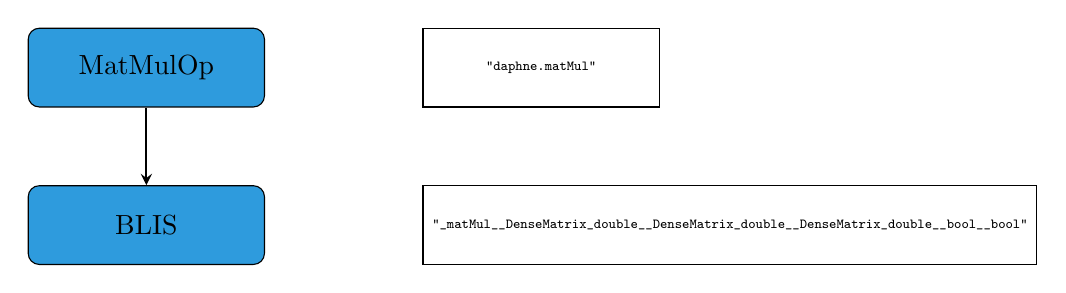
\begin{tikzpicture}[node distance=2cm]

\node (start) [startstop] {MatMulOp};
\node (matMulOp) [code, right = of start] {\tiny\Verb|"daphne.matMul"|};
\node (stop) [startstop, below of=start] {BLIS};
\node (blisMatMul) [code, right = of stop] {\tiny\Verb|"_matMul__DenseMatrix_double__|\Verb|DenseMatrix_double|\Verb|__DenseMatrix_double|\Verb|__bool__bool"|};


\draw [arrow] (start) -- (stop);

\end{tikzpicture}
\end{frame}

\begin{frame}{Daphne Matrix Multiplication -- Code Generation}
    Project outcomes:
    \begin{itemize}
\item    Enabled Matrix Multiplication for \Verb|ui64| value type\vs

    \item Extended code generation to \Verb|f32| and \Verb|si64|, \Verb|ui64| value types\vs

    \pause
    \item Enabled multiple Optimization strategies
    \end{itemize}
    \vs 

    \fullcite{udaybondhugulaUsingMLIRHighPerformance2020}\vs
\end{frame}

\begin{frame}{Matrix Multiplication}
    \centering
    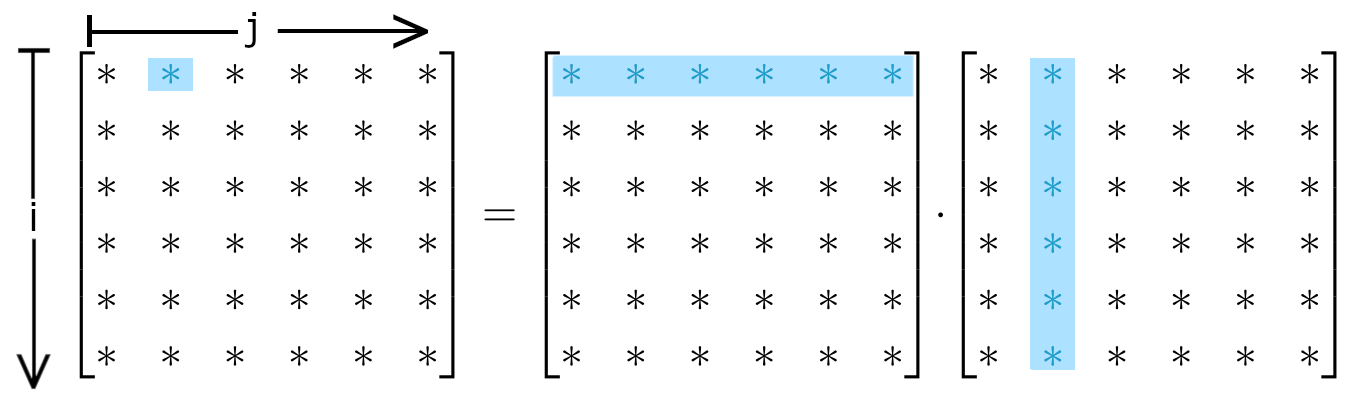
\includegraphics[width=\textwidth]{../Figures/matMulVecVecInd}
\end{frame}

\begin{frame}{Matrix Multiplication -- Inverted Loops}
    \centering
    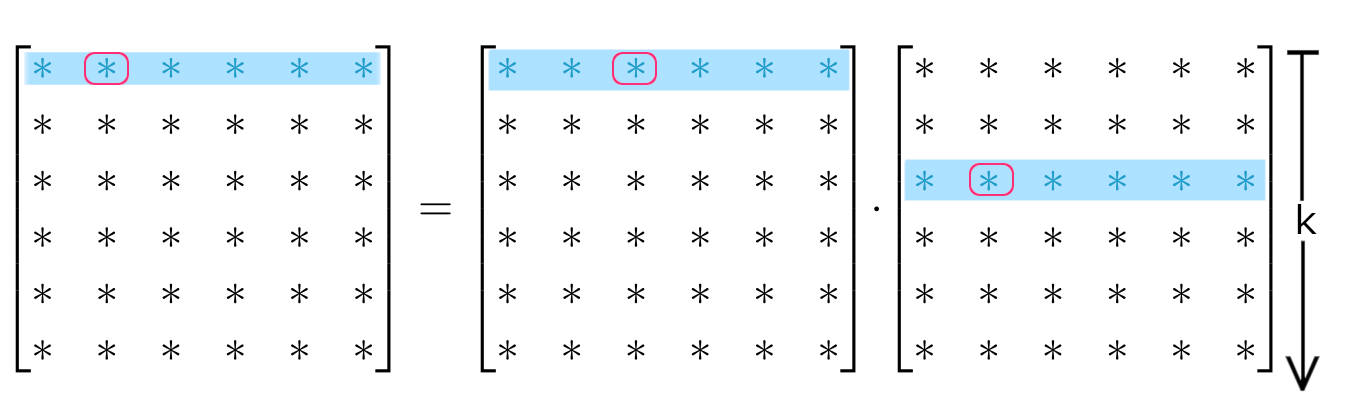
\includegraphics[width=\textwidth]{../Figures/matMulInvertedLoops}
\end{frame}

\begin{frame}{Matrix Multiplication -- Tiles and Vectors}
    \centering
    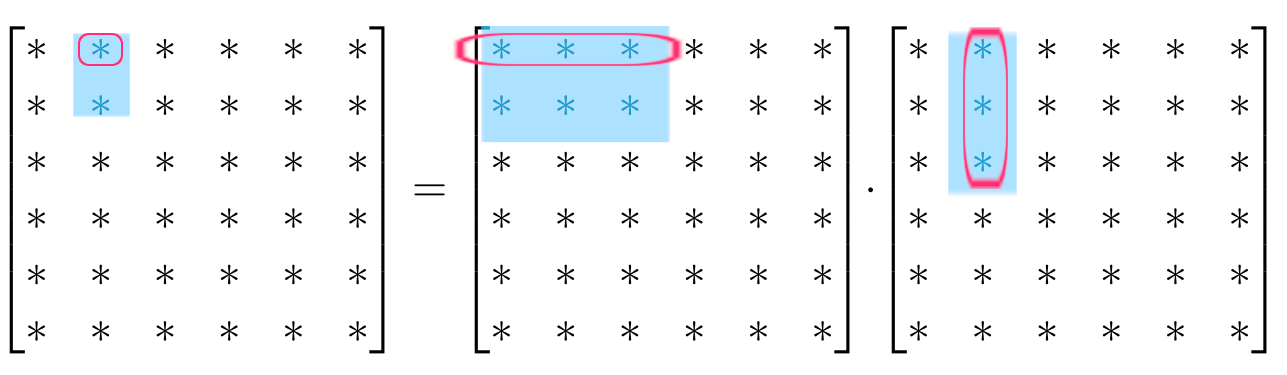
\includegraphics[width=\textwidth]{../Figures/matMulBond}
\end{frame}

\begin{frame}{Daphne Matrix Multiplication -- Code Generation}
    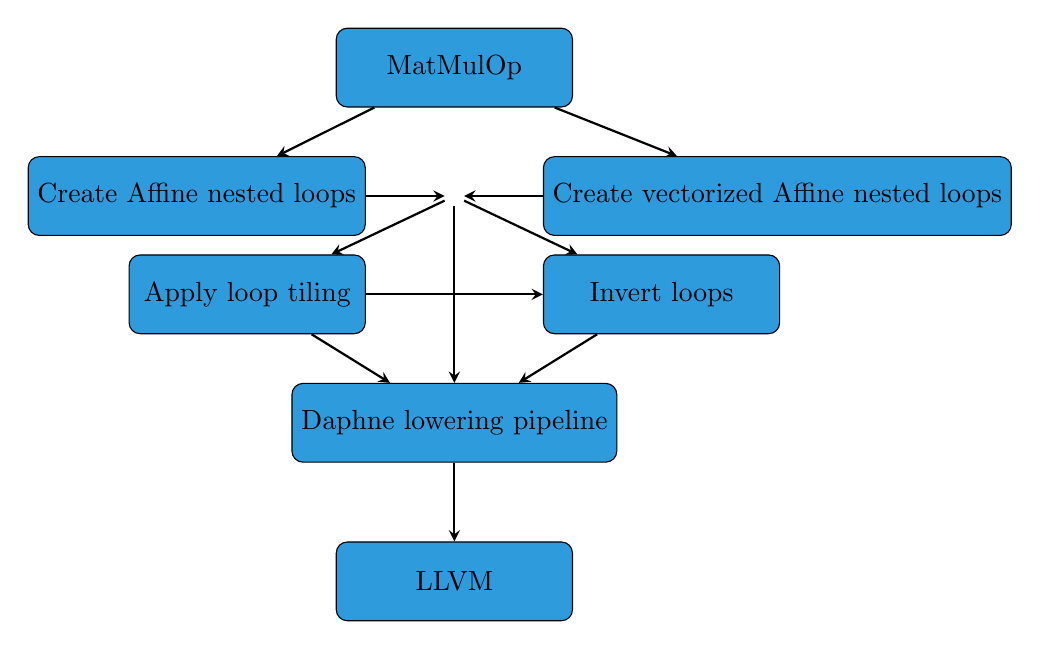
\begin{tikzpicture}[node distance=1cm]

\node (start) [startstop] {MatMulOp};
%\node (matMulOp) [code, right = of start] {\tiny\Verb|"daphne.matMul"|};

\node (affine) [below = of start] {};

\node (affineReg) [startstop, left = of affine] {Create Affine nested loops};
\node (affineVec) [startstop, right = of affine] {Create vectorized Affine nested loops};
%\node (affineCode) [code, right = of affine] {\tiny\Verb|AffineForOp| and \Verb|AffineLoadOp| or \Verb|AffineVectorLoadOp|};

\node (dummy) [below = of affine] {};
\node (tile) [startstop, left = of dummy] {Apply loop tiling};

\node (invert) [startstop, right = of dummy] {Invert loops};

\node (stop) [startstop, below = of dummy] {Daphne lowering pipeline};
%\node (affineFor) [code, right = of stop] {\tiny\Verb|affine.for|};

\node (llvm) [startstop, below = of stop] {LLVM};



\draw [arrow] (start) -- (affineReg);
\draw [arrow] (start) -- (affineVec);
\draw [arrow] (affineReg) -- (affine);
\draw [arrow] (affineVec) -- (affine);
\draw [arrow] (affine) -- (stop);
\draw [arrow] (affine) -- (tile);
\draw [arrow] (tile) -- (stop);
\draw [arrow] (tile) -- (invert);
\draw [arrow] (affine) -- (invert);
\draw [arrow] (invert) -- (stop);
\draw [arrow] (stop) -- (llvm);


\end{tikzpicture}
\end{frame}

\begin{frame}{Optimizations enabled}
    \begin{figure}
    \begin{minipage}{.45\textwidth}
        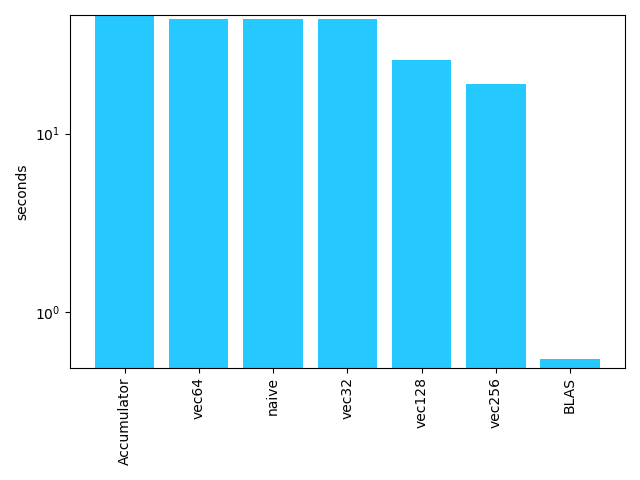
\includegraphics[width=\textwidth]{../Figures/vectorization}
    \end{minipage}
    \begin{minipage}{.45\textwidth}
        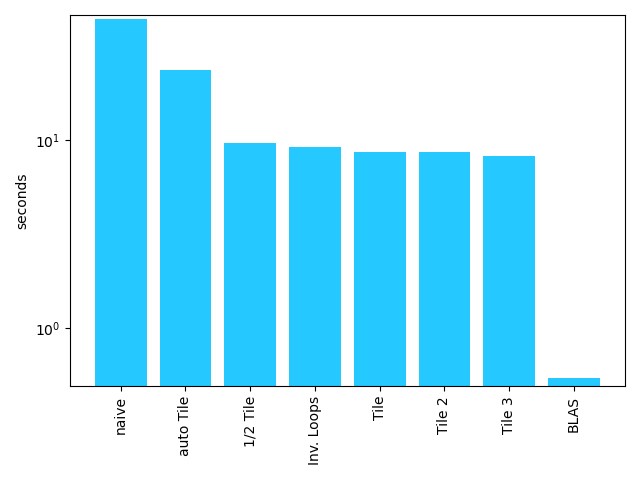
\includegraphics[width=\textwidth]{../Figures/tilingStrats}
    \end{minipage}
    \caption*{Execution times of dense $2048\times2048$ double precision Matrix multiplication with different 
    vector instruction sizes (left) and tiling strategies (right) enabled.}
\end{figure}
\end{frame}

\begin{frame}{Optimizations enabled -- Tiling and Vectorization}
    \begin{figure}
    \centering
    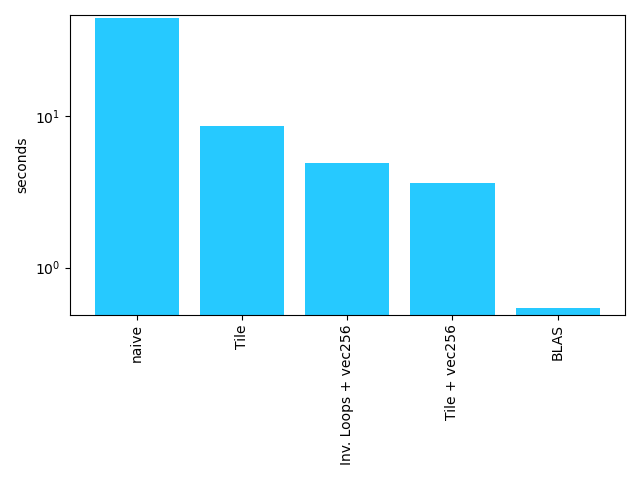
\includegraphics[height=.6\textheight]{../Figures/combinedVecTiling}
    \caption*{Execution times of dense $2048\times2048$ double precision Matrix multiplication with different optimizations.}
    \end{figure}
\end{frame}

\begin{frame}{Scaling behaviour}
    \begin{figure}
\centering
    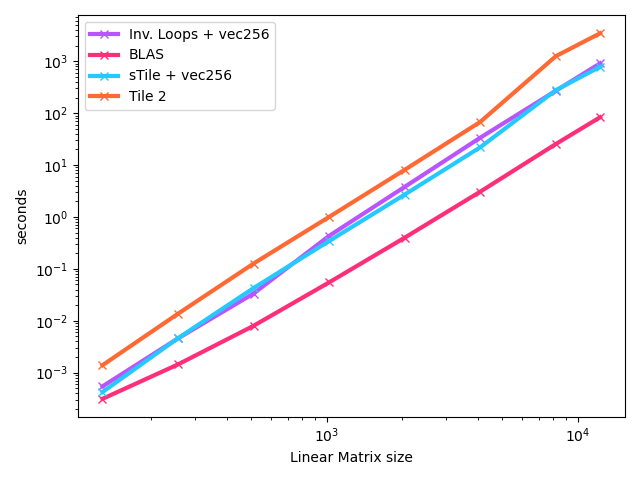
\includegraphics[height=.6\textheight]{../Figures/varSizesSubset}
    \caption*{Execution times of dense double precision Matrix multiplications.}
    \end{figure}
\end{frame}

\begin{frame}{Single precision Matrix Multiplication}
    \begin{figure}
    \centering
    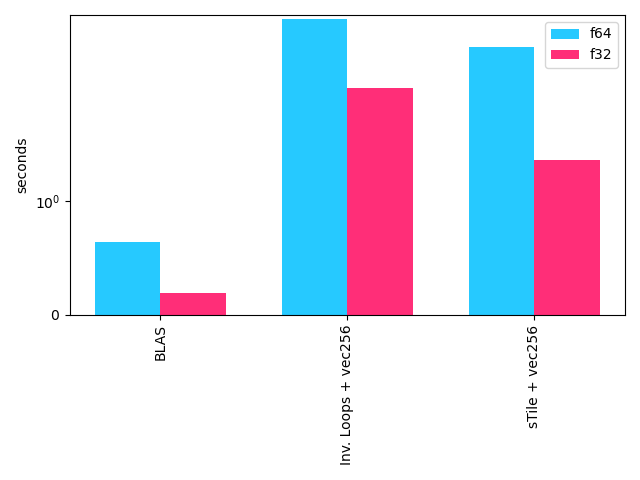
\includegraphics[height=.6\textheight]{../Figures/singleVsDouble}
    \caption*{Execution times of $2048\times2048$ dense single and double precision Matrix multiplications.}
    \end{figure}
\end{frame}

\begin{frame}{Further improvement -- Packing}
    \begin{figure}
    \centering
    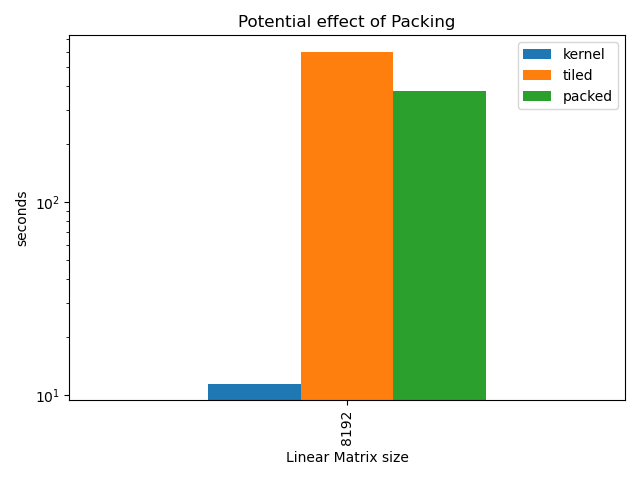
\includegraphics[height=.6\textheight]{../Figures/packing}
    \caption*{Effect of packing, enabled through \Verb|affineDataCopyGeneratePass|, on $8192\times8192$ single precision Matrix 
    multiplication executed with \Verb|mlir-cpu-runner|.}
    \end{figure}
\end{frame}

\begin{frame}[allowframebreaks,noframenumbering,plain]{Bibliography}
    \printbibliography
    % you can also put absolute paths here
\end{frame}

\begin{frame}[noframenumbering,plain]
    {\centering\usebeamerfont{title}\usebeamercolor[fg]{title}\insertauthor}%
\end{frame}

\begin{frame}{Appendix}
    \begin{figure}
    \centering
    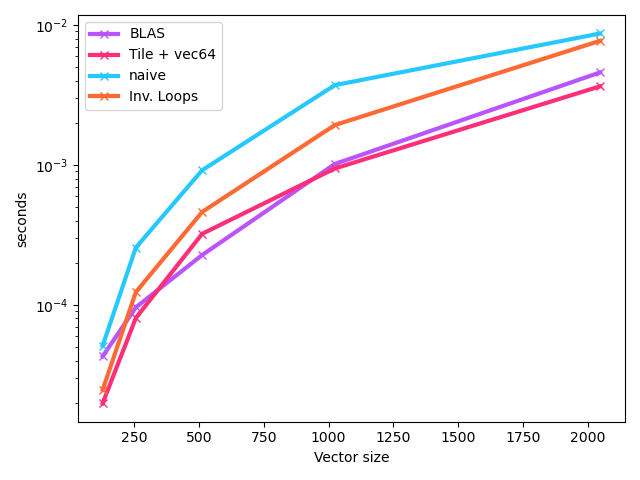
\includegraphics[height=.6\textheight]{../Figures/matVecSubset}
    \caption*{Execution times of double precision Matrix Vector product.}
    \end{figure}
\end{frame}


\begin{frame}[noframenumbering]{Appendix}
    \begin{figure}
    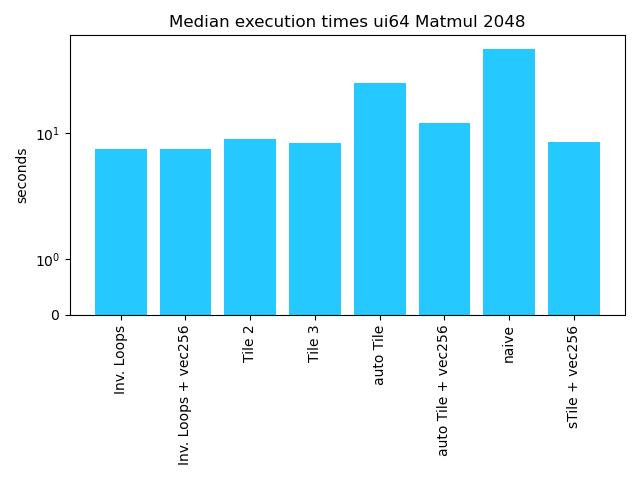
\includegraphics[height=.6\textheight]{../Figures/intExecution}
    \caption*{Exection times of ui64 $2048\times2048$ Matrix multiplication. Note this is not supported by
    the provided Kernel implementation.}
\end{figure}
\end{frame}

\begin{frame}[noframenumbering]{Appendix}
    \begin{figure}
    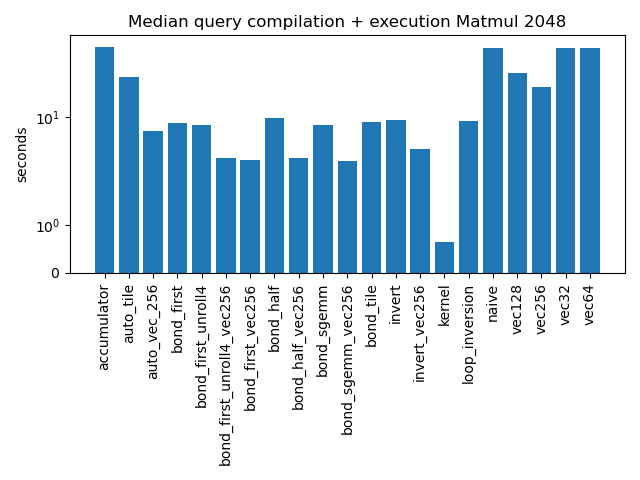
\includegraphics[height=.6\textheight]{../Figures/compilationExecution}
    \end{figure}
\end{frame}
\begin{frame}[noframenumbering]{Appendix}
    \begin{figure}
    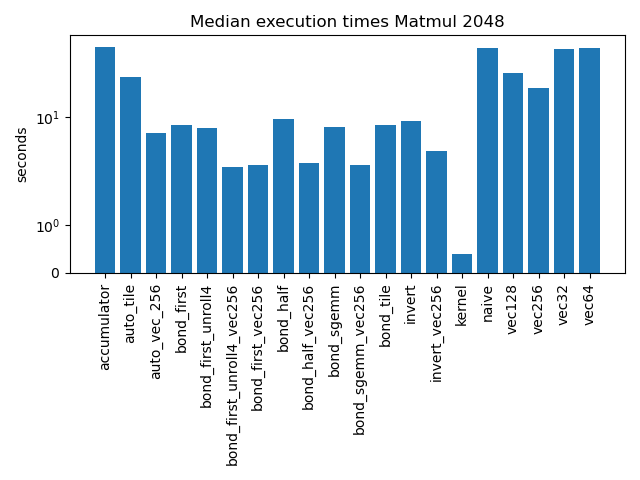
\includegraphics[height=.6\textheight]{../Figures/execution}
\end{figure}
\end{frame}
\begin{frame}[noframenumbering]{Appendix}
    \begin{figure}
    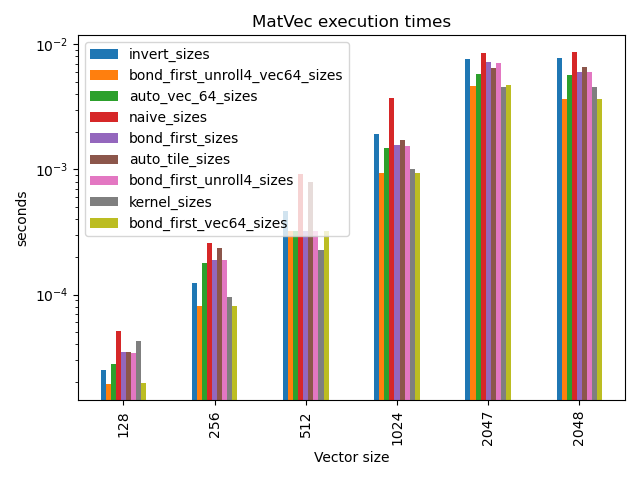
\includegraphics[height=.6\textheight]{../Figures/matVec}
\end{figure}
\end{frame}
\begin{frame}[noframenumbering]{Appendix}
    \begin{figure}
    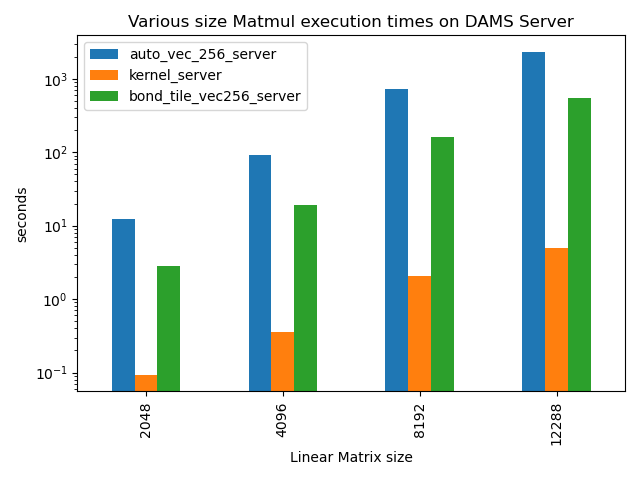
\includegraphics[height=.6\textheight]{../Figures/server}
\end{figure}
\end{frame}
\begin{frame}[noframenumbering]{Appendix}
    \begin{figure}
    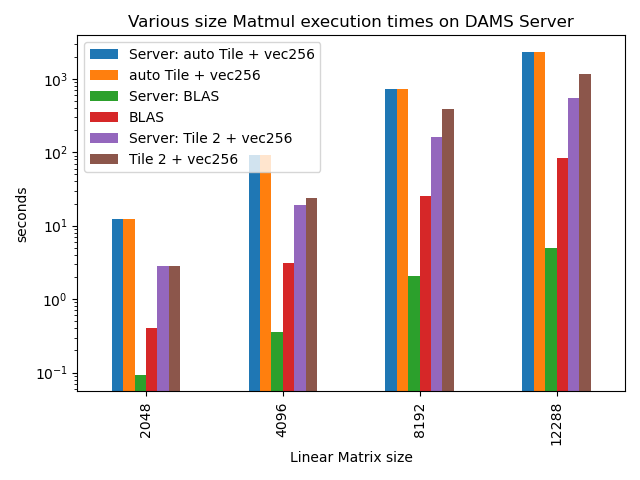
\includegraphics[height=.6\textheight]{../Figures/serverVsLocal}
\end{figure}
\end{frame}
\begin{frame}[noframenumbering]{Appendix}
    \begin{figure}
    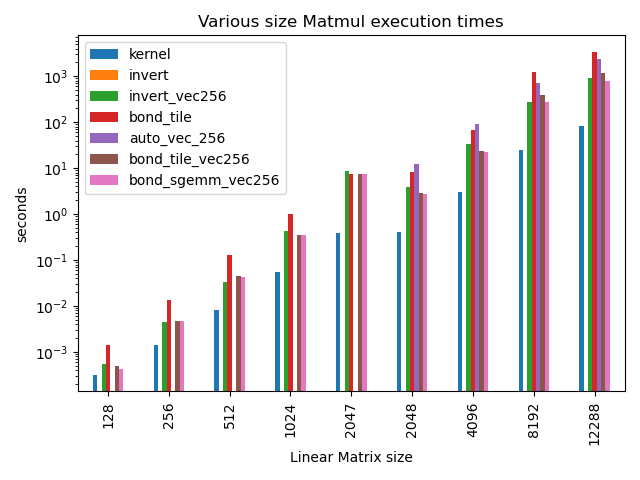
\includegraphics[height=.6\textheight]{../Figures/varSizes}
\end{figure}
\end{frame}
\end{document}